\documentclass[11pt]{article}

\usepackage[a4paper, total={6in, 8in}]{geometry}
\usepackage{graphicx}
\usepackage{multicol}
\usepackage{multirow}

\title{July2023 CSE300 Week10 Online Evaluation}
\author{Md. Emamul Haque Pranta}
\date{February 6, 2024}

\begin{document}
    \maketitle
    \tableofcontents
    \pagebreak
    
    \section{RISC Architecture}
    \begin{figure}[h]
        \centering
        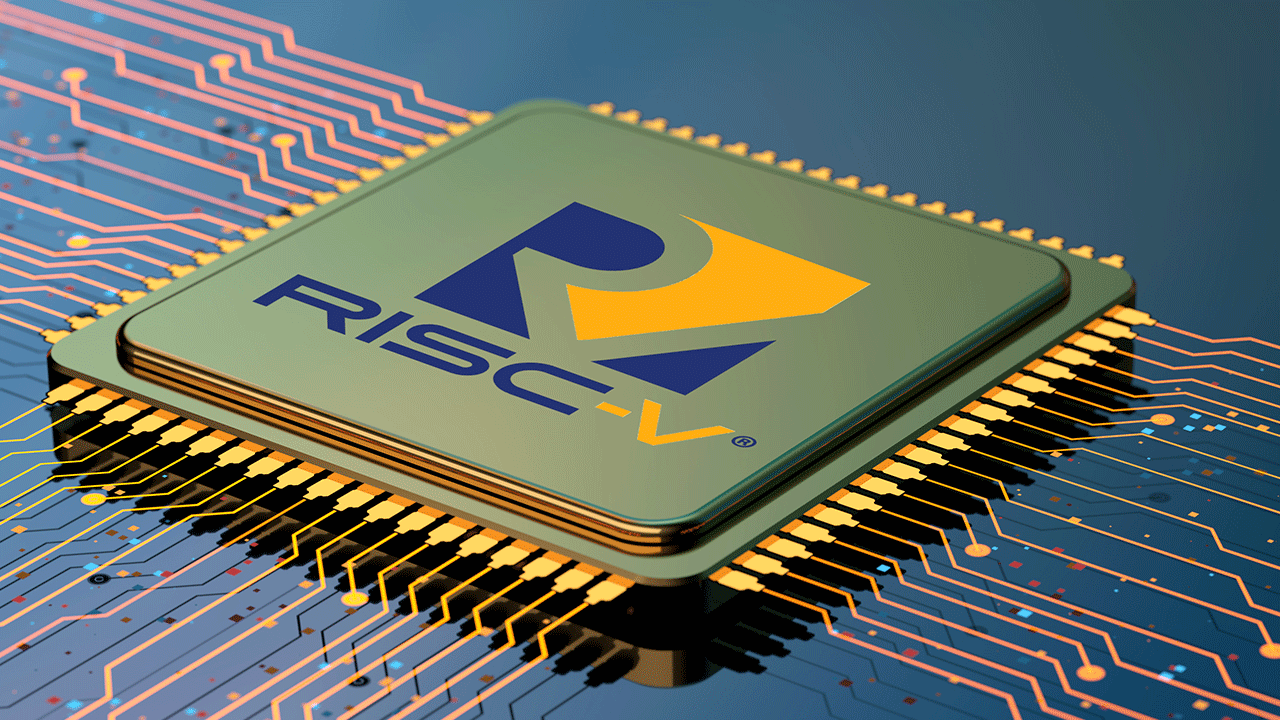
\includegraphics[scale=0.25]{images/risc.png}
        \caption{Risc architecture}
        \label{fig:enter-label}
    \end{figure}

    \section{Tables in LATEX}
    \begin{table}[h]
        \centering
        \begin{tabular}{c|c|c|c}
            \hline
            \multirow{6}{*}{numeric literals} & \multirow{3}{*}{integers} & in decimal & 8743 \\
            \hline
            \multirow{6}{*}{} &\multirow{3}{*}{} & in octal &0o7464\\
            \hline
            \multirow{6}{*}{} &\multirow{3}{*}{} & in hexadecimal &0O103\\
        \end{tabular}
        \caption{A table in LATEX}
        \label{tab:my_label}
    \end{table}

    Table 1 shows a table that contains cells spanning multiple columns and multiple rows.\cite{greedy}

    \section{Writing Equations in Latex}
    $L_split = \frac{1}{2}[\frac{G_L^2}{H_L+\lambda}+\frac{G_R^2}{H_R+\lambda}-\frac{(G_L+G_R)^2}{H_L+H_R+\lambda}]-\gamma$

    Equation 1 has been displayed above.\cite{random}


    \section*{Untitled Section}
    You need to display this section in your output PDF file. This section contains information that may help you prepare the bibliography section. By the way, this section will not show up in the table of contents.

    \begin{enumerate}
        \item Citation about the Greedy Forest Article
        \begin{itemize}
        \item \textbf{Authors:} T. Zhang, R. Johnson
        \item \textbf{Title:} Learning nonlinear functions using regularized greedy forest
        \item \textbf{Year:} 2014
        \item \textbf{Journal:} IEEE Transactions on Pattern Analysis and Machine Intelligence
        \end{itemize}

        \item Citation about the Random Forest Article
        \begin{itemize}
        \item \textbf{Author:} L. Breiman
        \item \textbf{Title:} Random Forests 
        \item \textbf{Journal:}Machine Learning
        \item \textbf{Year:} 2001
        \end{itemize}
        
    \end{enumerate}
    
    
    \bibliographystyle{plain}
    \bibliography{ref}
\end{document}